\section{基本概念}
\begin{enumerate}
    \item 考虑由约束
    \[x_1^2+x_2^2 \leqslant 1,\quad 1-x_2+x_1 \geqslant 0, \quad x_1 \leqslant 0\]确定的可行域$\mathcal{F}$. 判定点$\displaystyle x^{(1)}=\left(-\frac{1}{2},\frac{1}{2}\right)^{\mathrm{T}},x^{(2)}=(-1,1)^{\mathrm{T}},x^{(3)}=(-1,0)^{\mathrm{T}},x^{(4)}=\left(0,-\frac{1}{2}\right)^{\mathrm{T}}$和$\displaystyle x^{(5)}=\left(-\frac{1}{2},-\frac{1}{2}\right)^{\mathrm{T}}$是否是可行点? 如果是可行点,是内点还是边界点? 是哪个约束的边界点?\\
    \sol 画出可行域$\mathcal{F}$,图如下
    \begin{center}
        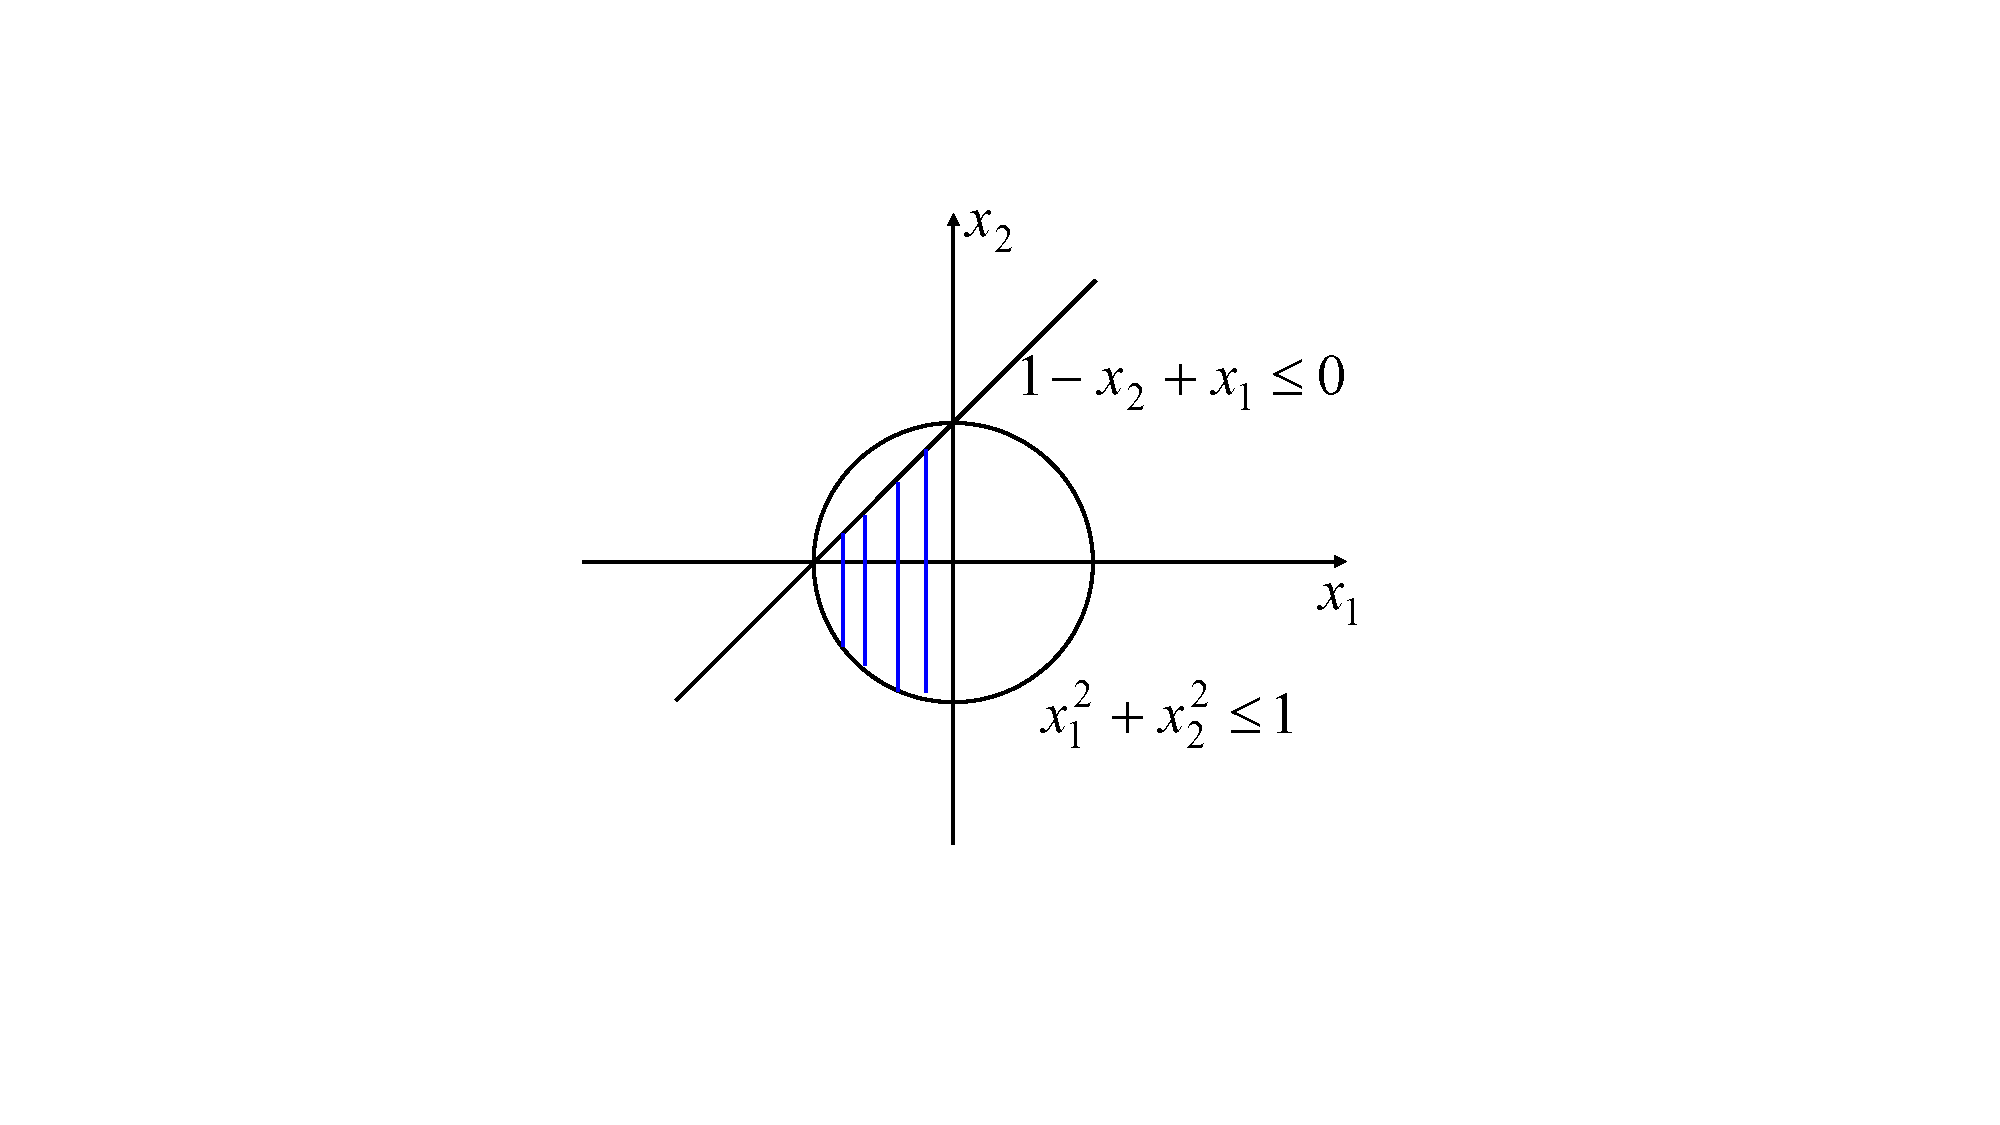
\includegraphics[scale=0.35]{1-1.pdf}
    \end{center}
    则$x^{(1)}$是可行点,是$1-x_2+x_1 \geqslant 0$的边界点;\\
    $x^{(2)}$不是可行点;\\
    $x^{(3)}$是可行点,是$x_1^2+x_2^2 \leqslant 1$和$1-x_2+x_1 \geqslant 0$的边界点;\\
    $x^{(4)}$是可行点,是$x_1 \leqslant 0$的边界点;\\
    $x^{(5)}$是可行点,也是内点.
    \item 考虑下述约束最优化问题
    \[\begin{cases}
        \min & x_1\\
        \mathrm{s.t.} & x_1^2+(x_2-2)^2 \leqslant 3,\\
        & x_1^2 \geqslant 1,
    \end{cases}\]
    画出问题的可行域和目标函数的等位线,并由此确定问题的所有局部最优解和全局最优解.\\
    \sol 可行域和等位线如下
    \begin{center}
        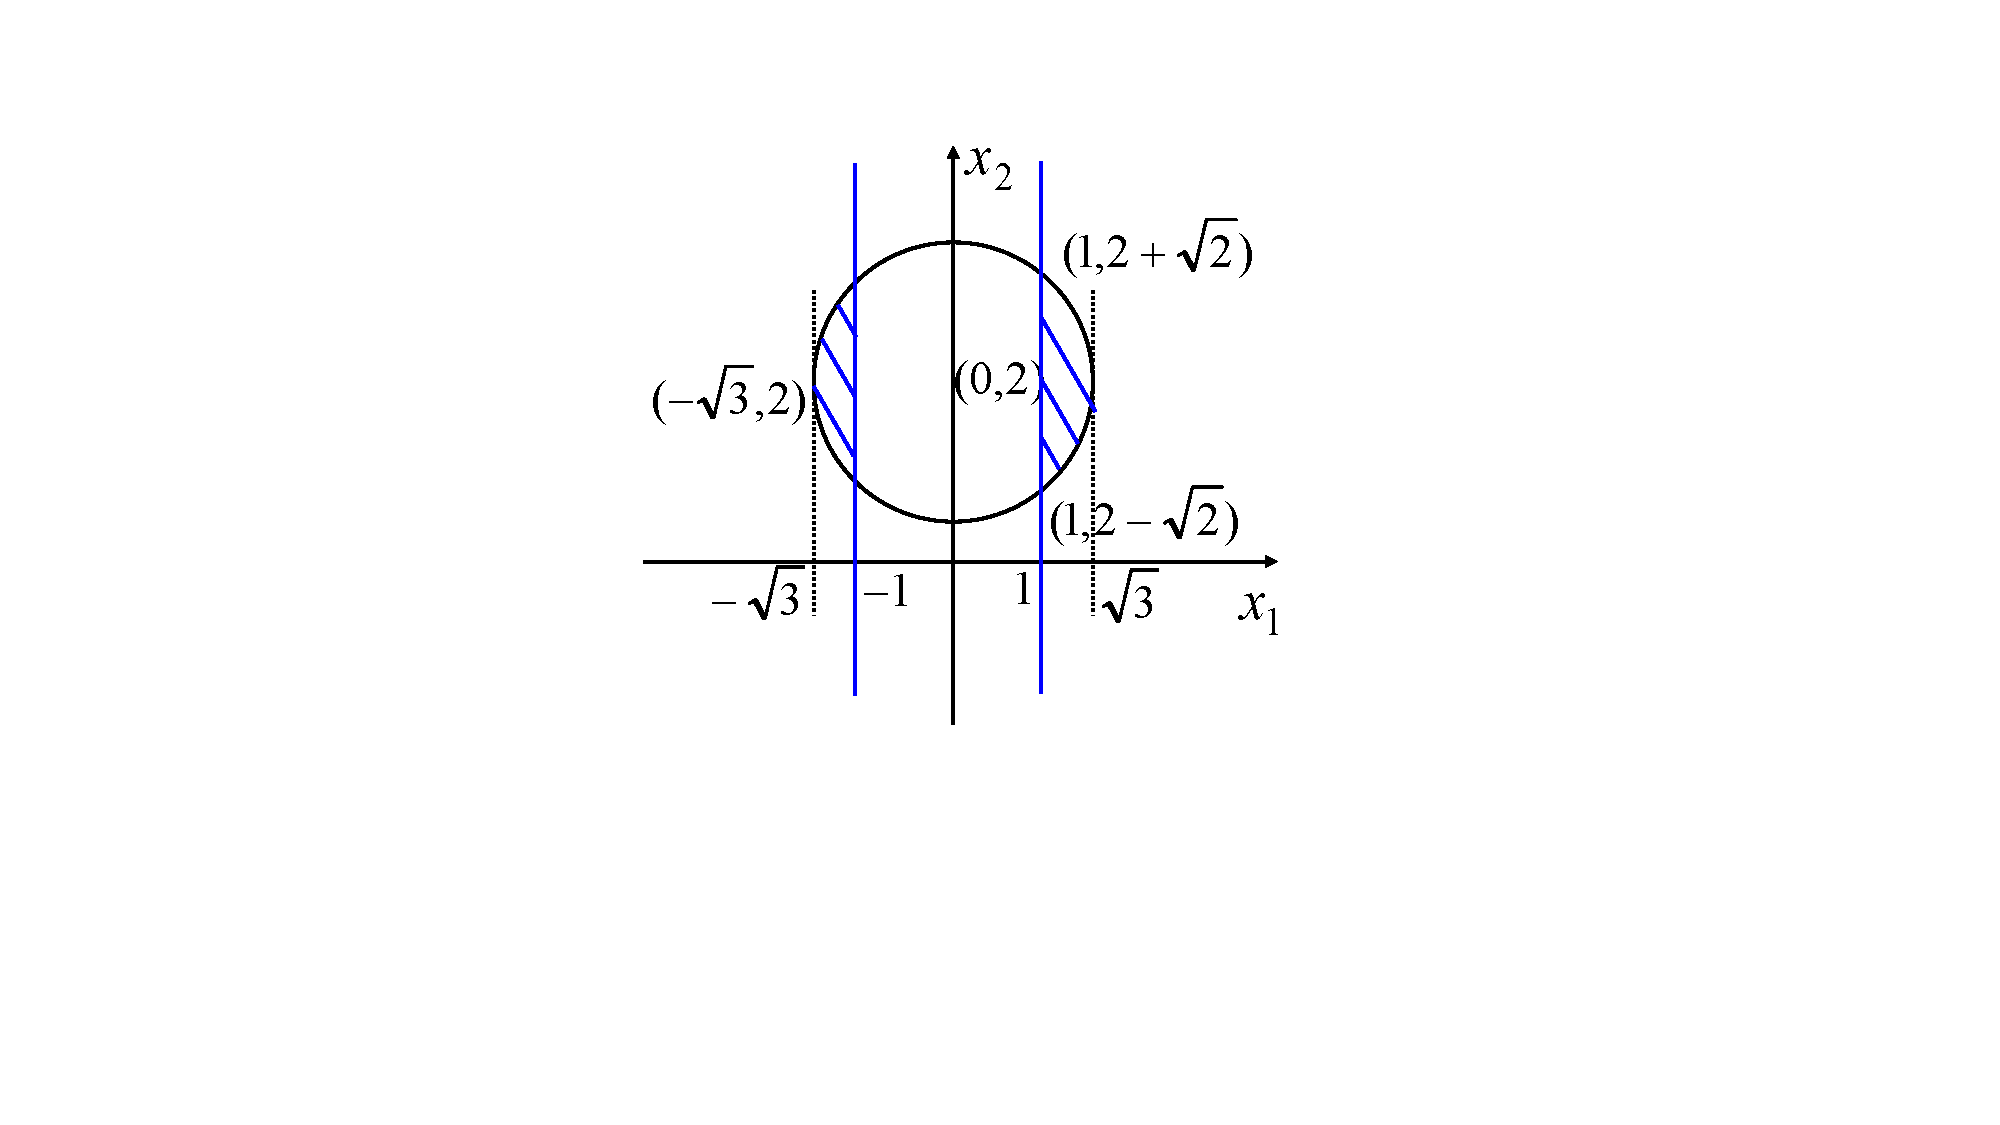
\includegraphics[scale=0.45]{1-2.pdf}
    \end{center}
    等位线:$f(x_1)=k$;局部最优解:$x_1=-\sqrt{3},x_2=2$和$x_1=1,x_2 \in [2-\sqrt{2},2+\sqrt{2}]$;\\全局最优解:$x_1=-\sqrt{3},x_2=2$.
    \item 设$\mathcal{F}=\{x \left| c_i(x) \geqslant 0,i=1,2,\cdots,m\right.\}$,其中所有$c_i(x)(i=1,2,\cdots,m)$都连续. 证明点$\bar{x} \in \mathcal{F}$是内点当且仅当对某一$\varepsilon>0$有\[\{x \left| ||x-\bar{x}|| < \varepsilon\right.\} \subset \mathcal{F}.\]
    \pro
    \[\bar{x}\text{是内点} \iff c_i(\bar{x}) > 0 \iff \forall \delta>0, U(A,\delta) \subset \mathcal{F} \iff \forall \varepsilon>0, \{x \left| ||x-\bar{x}|| < \varepsilon\right.\} \subset \mathcal{F}.\]
    \item \begin{enumerate}[label=(\arabic*)]
        \item 证明有限个凸集的交集仍然是凸集.
        \item 设$D_1=\{x|x_1+x_2 \leqslant 1, x_1 \geqslant 0\},D_2=\{x|x_1-x_2 \geqslant 0,x_1 \leqslant 0\}$. 令$D=D_1 \cup D_2$. 证明$D_1,D_2$均是凸集,但$D$却不是凸的,由此得出凸集的并集未必是凸集.
    \end{enumerate}
    \pro \begin{enumerate}[label=(\arabic*)]
        \item 设$\displaystyle C=\bigcap\limits_{i=1}^{n} C_i$,其中$C_i(i=1,2,\cdots,n)$均是凸集. 取$x_1,x_2 \in C$,则对于$\forall i$都有$x_1,x_2 \in C_i$. 取$\mu_1,\mu_2 \in [0,1]$且$\mu_1+\mu_2=1$,则有$\mu_1x_1+\mu_2x_2 \in C_i$. 因此有$\displaystyle \mu_1x_1+\mu_2x_2 \in \bigcap\limits_{i=1}^{n} C_i=C$,即$C$为凸集. 说明有限个凸集的交集仍然是凸集.
        \item 证明$D_1$是凸集:\\$\forall x,y \in D_1, x=(x_1,x_2), y=(y_1,y_2),\lambda \in [0,1],\lambda x + (1-\lambda)y =(\lambda x_1 + (1-\lambda)y_1,\lambda x_2 + (1-\lambda)y_2)$,
        \begin{align*}
            \lambda x_1 + (1-\lambda)y_1 + \lambda x_2 + (1-\lambda)y_2 & = \lambda (x_1+x_2)+(1-\lambda)(y_1+y_2)\\
            &\leqslant \lambda + 1 - \lambda =1
        \end{align*}
        $\lambda x_1 + (1-\lambda)y_1 \geqslant 0 \Rightarrow \lambda x + (1-\lambda)y \in D_1 \Rightarrow D_1$为凸集.\\
        证明$D_2$是凸集:\\$\forall x,y \in D_2, x=(x_1,x_2), y=(y_1,y_2),\lambda \in [0,1],\lambda x + (1-\lambda)y =(\lambda x_1 + (1-\lambda)y_1,\lambda x_2 + (1-\lambda)y_2)$,
        \begin{align*}
            \lambda x_1 + (1-\lambda)y_1 - \lambda x_2 - (1-\lambda)y_2 & = \lambda (x_1-x_2)+(1-\lambda)(y_1-y_2)\\
            &\geqslant 0
        \end{align*}
        $\lambda x_1 + (1-\lambda)y_1 \leqslant 0 \Rightarrow \lambda x + (1-\lambda)y \in D_2 \Rightarrow D_2$为凸集.\\
        证明$D$不是凸集:\\取$\displaystyle x=(1,0) \in D,y=(0,-1) \in D, \lambda =\frac{1}{2}$,则$\displaystyle \lambda x + (1-\lambda)y=\left(\frac{1}{2},-\frac{1}{2}\right) \not \in D \Rightarrow D$不是凸集.
    \end{enumerate}
    \item 设$u,v \in \textbf{R}^n$,对于2-范数$\| \cdot \|$,如果\[\|u+v\|=\|u\|+\|v\|,\]则$u=0$或$v=\lambda u$,对某个实数$\lambda$.\\
    \pro 向量的2-范数的定义为\[\|x\|_2=\left(\sum\limits_{i=1}^n x_i^2\right)^{\frac{1}{2}}.\]
    设$u=(u_1,u_2,\cdots,u_n),v=(v_1,v_2,\cdots,v_n)$. 对$\|u+v\|=\|u\|+\|v\|$两边平方,可得
    \begin{align*}
        \|u+v\|^2 & = \sum\limits_{i=1}^n (u_i+v_i)^2 \\
        & = \sum\limits_{i=1}^n (u_i+2u_iv_i+v_i^2) \\
        & = \sum\limits_{i=1}^n u_i^2 + 2\sum\limits_{i=1}^n u_iv_i + \sum\limits_{i=1}^n v_i^2 \\
        & = \|u\|^2 + 2\|u\|\|v\| + \|v\|^2\\
        & = \sum\limits_{i=1}^n u_i^2 + \sum\limits_{i=1}^n v_i^2 +\sqrt{\sum\limits_{i=1}^n u_i^2 \cdot \sum\limits_{i=1}^n v_i^2}
    \end{align*}
    即\[\left(\sum\limits_{i=1}^n u_iv_i\right)^2 = \sum\limits_{i=1}^n u_i^2 \cdot \sum\limits_{i=1}^n v_i^2,\]
    而由柯西不等式\[\left(\sum\limits_{i=1}^n u_iv_i\right)^2 \leqslant \sum\limits_{i=1}^n u_i^2 \cdot \sum\limits_{i=1}^n v_i^2,\]
    当且仅当$\displaystyle \frac{v_1}{u_1}=\frac{v_2}{u_2}=\cdots=\frac{v_n}{u_n} = \lambda (\lambda \neq 0)$或$u_i,v_i$其中一方全为0时,取到等号,即$u=0$或$v = \lambda u$.
    \item 设$f(x)$为定义在凸集$D \subset \textbf{R}^n$上的凸函数,$\alpha$为一个给定的实数,称集合\[\mathcal{T}=\{x|f(x) \leqslant \alpha\}\]为函数$f(x)$关于实数$\alpha$的水平集. 证明对任意实数$\alpha$,集合$\mathcal{T}$是凸集.\\
    \pro 对于$\forall x_1,x_2 \in \mathcal{T}$,根据$\mathcal{T}$的定义则有$f(x_1) \leqslant \alpha,f(x_2) \leqslant \alpha$. 由于$D$是凸集,则对于$\forall \lambda \in [0,1]$,必有\[\lambda x_1 + (1-\lambda)x_2 \in D\]
    又由于$f(x)$是$D$上的凸函数,则有
    \begin{align*}
        f\left(\lambda x_1 + (1-\lambda)x_2\right) & \leqslant \lambda f(x_1) + (1-\lambda)f(x_2)\\
        & \leqslant \lambda \alpha + (1-\lambda)\alpha = \alpha
    \end{align*}
    因此$\lambda x_1 + (1-\lambda)x_2 \in \mathcal{T}$,故对任意实数$\alpha$,集合$\mathcal{T}$是凸集.
    \item 设$f_i(x)(i=1,2,\cdots,m)$是定义在凸集$D \subset \textbf{R}^n$上的凸函数,证明函数\[g(x)=\sum\limits_{i=1}^m \alpha_if_i(x)\]也是$D$上的凸函数,其中$\displaystyle \sum\limits_{i=1}^m \alpha_i=1,\alpha_i \geqslant 0(i=1,2,\cdots,m)$,即凸函数的组合还是凸函数.\\
    \pro 对于$\forall x,y \in D,\lambda \in [0,1]$,由于$\displaystyle \sum\limits_{i=1}^m \alpha_i=1,\alpha_i \geqslant 0(i=1,2,\cdots,m)$,则有
    \begin{align*}
        g(\lambda x+(1-\lambda)y) & = \sum\limits_{i=1}^m \alpha_if_i(\lambda x+(1-\lambda)y)\\
        & \leqslant \sum\limits_{i=1}^m \alpha_i[\lambda f_i(x)+(1-\lambda)f_i(y)]\\
        &=\lambda \sum\limits_{i=1}^m \alpha_if_i(x)+(1-\lambda)\sum\limits_{i=1}^m \alpha_if_i(y)\\
        &=\lambda g(x) + (1-\lambda) g(y)
    \end{align*}
    则$\displaystyle g(x)=\sum\limits_{i=1}^m \alpha_if_i(x)$也是$D$上的凸函数.
    \item 设$c_i(x)(i \in E)$是线性函数,$c_i(x)(i \in I)$是凹函数,证明约束集\[\varOmega=\left\{x\left|\begin{array}{cc}\begin{matrix}c_i(x)=0, & i \in E\\c_i(x)\geqslant 0, & i \in I \end{matrix}\end{array}\right.\right\}\]是凸集.\\
    \pro $\forall x_1,x_2 \in \varOmega, \lambda \in [0,1]$,则可以分成以下三种情况:
    \begin{enumerate}[label=(\arabic*)]
        \item 若$c_i(x_1)=0,c_i(x_2)=0$,则
        \[c_i(\lambda x_1 + (1-\lambda)x_2) = \lambda c_i(x_1) + (1- \lambda)c_i(x_2) = 0 \Rightarrow \lambda x_1 + (1-\lambda)x_2 \in \varOmega,\]
        故$\varOmega$是凸集.
        \item 若$c_i(x_1)\geqslant 0,c_i(x_2)\geqslant 0$,则
        \[-c_i(\lambda x_1 + (1-\lambda)x_2) \leqslant -\lambda c_i(x_1) - (1- \lambda)c_i(x_2) \leqslant 0 \Rightarrow \lambda x_1 + (1-\lambda)x_2 \in \varOmega,\]
        故$\varOmega$是凸集.
        \item 若$c_i(x_1)= 0,c_i(x_2)\geqslant 0$(当$x_1,x_2$互换时,与此情况同理),则
        \[-c_i(\lambda x_1 + (1-\lambda)x_2) \leqslant -\lambda c_i(x_1) - (1- \lambda)c_i(x_2) = - (1- \lambda)c_i(x_2) \leqslant 0 \Rightarrow \lambda x_1 + (1-\lambda)x_2 \in \varOmega,\]
        故$\varOmega$是凸集.
    \end{enumerate}
    综上,约束集$\varOmega$是凸集.
    \item 设多变量函数$f: \textbf{R}^n \to \textbf{R}^1$和单变量函数$\phi: \textbf{R}^1 \to \textbf{R}^1$都是凸函数,证明复合函数$h(x)=\phi(f(x)),x \in \textbf{R}^n$是凸函数. \textcolor{red}{(补充:函数$\phi$单调非减)}\\
    \pro $\because f$是凸函数,$\forall x,y \in \textbf{R}^n, \lambda \in [0,1]$,\[\therefore f(\lambda x+(1-\lambda)y \leqslant \lambda f(x) + (1-\lambda)f(y).\]
    \begin{align*}
        h(\lambda x+(1-\lambda)y) & =\phi(f(\lambda x+(1-\lambda)y)\\
        & \leqslant \phi(\lambda f(x) + (1-\lambda)f(y)) \quad (\text{函数}\phi\text{单调非减})\\
        & \leqslant \lambda \phi(f(x)) + (1-\lambda)\phi(f(y)) \quad (\text{函数}\phi\text{是凸函数})\\
        & = \lambda h(x) + (1-\lambda)h(y)
    \end{align*}
    则复合函数$h(x)=\phi(f(x)),x \in \textbf{R}^n$是凸函数.
    \item 设$c_i(x)(i=1,2,\cdots,m)$为$\textbf{R}^n$上的凹函数,$f(x)$是$\textbf{R}^n$上的凸函数,证明函数\[P(x)=f(x)-\mu\sum\limits_{i=1}^m \log c_i(x)\]在集合$D=\{x | c_i(x) > 0\}$上是凸函数. \textcolor{red}{(补充:$\mu>0$)}\\
    \pro 易证:$\log c_i(x)$是凹函数,所以$\forall x,y \in D$,则
    \begin{align*}
        P(\lambda x+(1-\lambda)y) & = f(\lambda x+(1-\lambda)y)-\mu\sum\limits_{i=1}^m \log c_i(\lambda x+(1-\lambda)y)\\
        & \leqslant \lambda f(x) + (1-\lambda) f(y) - \mu\sum\limits_{i=1}^m \log (\lambda c_i(x)+(1-\lambda)c_i(y))\\
        & \leqslant \lambda f(x) + (1-\lambda) f(y) - \lambda\mu\sum\limits_{i=1}^m \log c_i(x)-(1-\lambda)\mu\sum\limits_{i=1}^m \log c_i(y)\\
        & = \lambda P(x) + (1-\lambda) P(y)
    \end{align*}
    所以,该函数在集合$D=\{x | c_i(x) > 0\}$上是凸函数.
    \item 设$A$是$m \times n$矩阵,$b$是$n$维向量,利用Farkas引理证明下述两组系统中有且仅有一组有解: \begin{align*}
        &Ax \leqslant 0, x \geqslant 0, b^{\mathrm{T}}x > 0;\\
        &A^{\mathrm{T}}y=b,y \geqslant 0.
    \end{align*}
    \pro 先给这个系统标号:
    \begin{align*}
        &Ax \leqslant 0, x \geqslant 0, b^{\mathrm{T}}x > 0; \quad (1)\\
        &A^{\mathrm{T}}y=b,y \geqslant 0; \quad (2)
    \end{align*}
    要证(1)(2)中有且仅有一组解,即证(1)有解$\iff$(2)无解。\\
    先证充分性:若(1)有解,则说明$\exists \bar{x} \geqslant 0$使得$A\bar{x} \leqslant 0,b^{\mathrm{T}} \bar{x}>0$. 用反证法证明(2)无解,若在(1)的条件下,(2)有解,则$\exists \bar{y} \geqslant 0$使得$A^{\mathrm{T}}\bar{y}=b$,即$\bar{y}^{\mathrm{T}}A=b^{\mathrm{T}}$,两边同时右乘$\bar{x}$,则有
    \[\bar{y}^{\mathrm{T}}A\bar{x}=b^{\mathrm{T}}\bar{x},\]
    由于$\bar{y} \geqslant 0, A\bar{x} \leqslant 0$,则$\bar{y}^{\mathrm{T}}A\bar{x} = b^{\mathrm{T}}\bar{x} \leqslant 0$,与(1)的$b^{\mathrm{T}} \bar{x}>0$矛盾,则若(1)有解,则(2)无解.\\
    再证必要性:若(2)无解,令$D=\{z | z=A^{\mathrm{T}}y, y \geqslant 0\}$,则$D \subset \textbf{R}^n$为非空闭凸集. 由定理1.2.6,$\exists a \in \textbf{R}^n(a \geqslant 0),\beta \in \textbf{R}$使得\[a^{\mathrm{T}}x \leqslant \beta < a^{\mathrm{T}}b,\quad \forall x \in D,\]
    由于$0 \in D$,则可知$\beta \geqslant 0, a^{\mathrm{T}}b > 0$. 同时\[\beta \geqslant a^{\mathrm{T}}x = a^{\mathrm{T}}A^{\mathrm{T}}y=y^{\mathrm{T}}Aa, \quad \forall y \geqslant 0,\]
    由于$y \geqslant 0$可以任意大,则$Aa \leqslant 0$,即$a$是(1)的解,则若(2)无解,则(1)有解. 证毕.
    \item 设$x^*$是凸规划问题的一个解. 证明如果目标函数严格凸,则$x^*$是唯一全局最优解.\\
    \pro 先证$x^*$是一个全局最优解:设$x^*$是凸规划问题的一个解(即局部最优解),但不是全局最优解,则$\exists y$满足$f(y)<f(x^*)$. 由可行域的凸性,对于$\lambda \in [0,1]$,点$\lambda x^*+(1-\lambda)y$都是可行点. 又根据目标函数的凸性有
    \begin{align*}
        f(\lambda x^*+(1-\lambda)y) & \leqslant \lambda f(x^*) + (1-\lambda)f(y)\\
        & \leqslant \lambda f(x^*) + (1-\lambda)f(x^*) = f(x^*)
    \end{align*}
    这表明在$x^*$的任意小的邻域内都存在函数值小于$f(x^*)$的可行点,这与$x^*$是局部最优解相矛盾,则$x^*$是一个全局最优解.\\
    再证$x^*$是唯一的:由于目标函数是严格凸的,设$x^* \neq y^*$都是全局最优解,则$f(x^*)=f(y^*)$. 由严格凸函数的定义,而$\forall \lambda \in (0,1)$,有
    \[f(\lambda x^*+(1-\lambda)y^*) < \leqslant \lambda f(x^*) + (1-\lambda)f(y^*) = f(x^*).\]
    这与$x^*$是全局最优解矛盾,则$x^*$是唯一的. 综上,$x^*$是唯一全局最优解.
    \item 设$f(x)$定义在集合$D \subset \textbf{R}^n$上且连续可微.
    \begin{enumerate}[label=(\arabic*)]
        \item 证明$f(x)$是$D$上严格凸函数的充分必要条件为\[f(y)>f(x)+ \nabla f(x)^{\mathrm{T}} (y-x),\quad\forall x,y \in D,x \neq y.\]
        \item 证明$f(x)$是$D$上一致凸函数的充分必要条件为\[f(y) \geqslant f(x)+ \nabla f(x)^{\mathrm{T}} (y-x) + c\|y-x\|^2,\quad\forall x,y \in D,\]其中$c>0$是某个常数. \textcolor{red}{(补充:$c$应该$<0$)}
    \end{enumerate}
    \pro \begin{enumerate}[label=(\arabic*)]
        \item 必要性:因为$f(x)$是严格凸函数,则对$\forall \lambda \in (0,1)$,有
        \[f(\lambda x+(1-\lambda)y) < \lambda f(x) + (1-\lambda) f(y),\]
        即
        \[f(x + \lambda(y-x)) < f(x) + \lambda(f(y)-f(x)).\]
        由泰勒公式,有\[f(x + \lambda(y-x)) = f(x) + \lambda \nabla f(x)^{\mathrm{T}} (y-x)+o(\|\lambda(y-x)\|).\]
        因此得到\[f(y)-f(x) > \nabla f(x)^{\mathrm{T}} (y-x)+\frac{o(\|\lambda(y-x)\|)}{\lambda}.\]
        令$\lambda \to 0^+$,则
        \[f(y)>f(x)+ \nabla f(x)^{\mathrm{T}} (y-x),\quad\forall x,y \in D,x \neq y.\]
        必要性得证.\\
        充分性:令$z=\lambda x+(1-\lambda)y$,则
        \[f(x) > f(z) + \nabla f(z)^{\mathrm{T}} (x-z),\]
        同理\[f(y) > f(z) + \nabla f(z)^{\mathrm{T}} (y-z),\]
        从而\[\lambda f(x) + (1-\lambda)f(y)-f(z) > \nabla f(z)^{\mathrm{T}} [\lambda(x-z) + (1-\lambda)(y-z)] = 0\]
        即\[f(\lambda x+(1-\lambda)y) < \lambda f(x) + (1-\lambda) f(y).\]
        充分性得证.
        \item 一致凸函数的定义为:$f(x)$是定义在$D$上的实值函数,若存在$k>0$,对$\forall x,y \in D, \lambda \in [0,1]$,有
        \[f(\lambda x+(1-\lambda)y) \leqslant \lambda f(x) + (1-\lambda) f(y) +k\lambda (1-\lambda) \|x-y\|^2,\]
        则称$f(x)$是$D$上的一致凸函数.\\
        必要性:因为$f(x)$是一致凸函数,则
        \[f(\lambda x+(1-\lambda)y) \leqslant \lambda f(x) + (1-\lambda) f(y) +k\lambda (1-\lambda) \|x-y\|^2,\]
        即
        \[f(x + \lambda(y-x)) \leqslant f(x) + \lambda(f(y)-f(x))+k\lambda (1-\lambda) \|x-y\|^2.\]
        由泰勒公式,有\[f(x + \lambda(y-x)) = f(x) + \lambda \nabla f(x)^{\mathrm{T}} (y-x)+o(\|\lambda(y-x)\|).\]
        因此得到\[f(y)-f(x) \geqslant \nabla f(x)^{\mathrm{T}} (y-x)+\frac{o(\|\lambda(y-x)\|)}{\lambda} - k(1-\lambda)\|x-y\|^2.\]
        令$\lambda \to 0^+$,则
        \[f(y) \geqslant f(x)+ \nabla f(x)^{\mathrm{T}} (y-x) - k\|x-y\|^2,\]
        令$c = -k < 0$,则
        \[f(y) \geqslant f(x)+ \nabla f(x)^{\mathrm{T}} (y-x) + c\|y-x\|^2,\quad\forall x,y \in D,x \neq y.\]
        必要性得证.\\
        充分性:令$z=\lambda x+(1-\lambda)y$,则
        \[f(x) \geqslant f(z) + \nabla f(z)^{\mathrm{T}} (x-z) + c\|x-z\|^2,\]
        同理\[f(y) \geqslant f(z) + \nabla f(z)^{\mathrm{T}} (y-z) + c\|y-z\|^2,\]
        从而
        \begin{align*}
            \lambda f(x) + (1-\lambda)f(y)-f(z) & \geqslant \nabla f(z)^{\mathrm{T}} [\lambda(x-z) + (1-\lambda)(y-z)] + c\lambda\|x-z\|^2 + c(1-\lambda)\|y-z\|^2\\
            &\geqslant 0 + c\lambda\|x-z\|^2 + c(1-\lambda)\|y-z\|^2 \\
            &\geqslant c\lambda(1-\lambda)\|y-x\|^2
        \end{align*}
        令$k = -c > 0$,则
        \[f(\lambda x+(1-\lambda)y) \leqslant \lambda f(x) + (1-\lambda) f(y) +k\lambda (1-\lambda) \|x-y\|^2.\]
        充分性得证.
    \end{enumerate}
    \item 求出函数\[f(x)=2x_1^3-3x_1^2-6x_1x_2(x_1-x_2-1)\]的所有稳定点,其中哪一个点是极小值点? 哪一个点是极大值点? 有没有既不是极大又不是极小的点?\\
    \sol $\displaystyle \nabla f=\left(\begin{array}{cc}
        \begin{matrix}
            6x_1^2-6x_1-12x_1x_2+6x_2^2+6x_2\\x_1(-6x_1+12x_2+6)
        \end{matrix}
    \end{array}\right)=\left(\begin{array}{cc}
        \begin{matrix}
            0 \\ 0
        \end{matrix}
    \end{array}\right),$\\
    $\displaystyle \nabla^2f=\left(\begin{array}{cc}
        \begin{matrix}
            12x_1-6-12x_2 & -12x_1+12x_2+6\\-12x_1+12x_2+6 & 12x_1
        \end{matrix}
    \end{array}\right)$,则所有稳定点为
    \[\left(\begin{array}{cc}
        \begin{matrix}
            0 \\ 0
        \end{matrix}
    \end{array}\right),\left(\begin{array}{cc}
        \begin{matrix}
            0 \\ -1
        \end{matrix}
    \end{array}\right),\left(\begin{array}{cc}
        \begin{matrix}
            -1 \\ -1
        \end{matrix}
    \end{array}\right),\left(\begin{array}{cc}
        \begin{matrix}
            1 \\ 0
        \end{matrix}
    \end{array}\right).\]
    依次代入$\nabla^2 f$,分别使得$\nabla^2 f$为不定,不定,负定,正定,则依次为非极大极小点,非极大极小点,局部极大点,局部极小点.
    \item 确定线性函数$f(x)=2x_1-x_2+3x_3$的所有下降方向. 请问这样的下降方向是否同所在点的位置有关?\\
    \sol $\displaystyle \nabla f(x)^{\mathrm{T}}=(2,-1,3)$,则$\nabla f(x)^{\mathrm{T}} s < 0$,设$s=(s_1,s_2,s_3)^{\mathrm{T}}$,则\[2s_1-s_2+3s_3 < 0,\]
    故函数$f(x)=2x_1-x_2+3x_3$的所有下降方向为$\mathcal{D}(x)=\{s | 2s_1-s_2+3s_3 < 0, s=(s_1,s_2,s_3)^{\mathrm{T}}\}$. 这样的下降方向与所在点的位置无关.
    \item 考虑约束最优化问题\[\begin{cases}
        \min & -x_1+x_2\\
        \mathrm{s.t.} & x_1+2x_2 \leqslant 2,\\
        & x_1 \geqslant 0, x_2 \geqslant 0,
    \end{cases}\]
    \begin{enumerate}[label=(\arabic*)]
        \item 确定在点$\displaystyle x^{(1)}=(0,0)^{\mathrm{T}},x^{(2)}=(0,1)^{\mathrm{T}},x^{(3)}=\left(1,\frac{1}{2}\right)^{\mathrm{T}}$和$x^{(4)}=(2,0)^{\mathrm{T}}$处的可行方向.
        \item 在这些点是否存在可行的下降方向,并由此从中确定最优解.
    \end{enumerate}
    \sol 本题需要教材7.1节的知识.\\
    先将所求化为标准形式:
    \[\begin{cases}
        \min & -x_1+x_2\\
        \mathrm{s.t.} & 2-x_1-2x_2 \geqslant 0,\\
        & x_1 \geqslant 0, x_2 \geqslant 0,
    \end{cases}\]
    \begin{enumerate}[label=(\arabic*)]
        \item 对于$x^{(1)}=(0,0)^{\mathrm{T}}$,有
        \[\begin{cases}
            d^{(1)\,\mathrm{T}} \left(\begin{array}{cc}
                \begin{matrix}
                    1\\0
                \end{matrix}
            \end{array}\right) \geqslant 0,\\
            d^{(1)\,\mathrm{T}} \left(\begin{array}{cc}
                \begin{matrix}
                    0\\1
                \end{matrix}
            \end{array}\right) \geqslant 0,
        \end{cases} \Rightarrow d_1^{(1)} \geqslant 0, d_2^{(1)} \geqslant 0, d^{(1)} \neq 0;\]
        对于$x^{(2)}=(0,1)^{\mathrm{T}}$,有
        \[\begin{cases}
            d^{(2)\,\mathrm{T}} \left(\begin{array}{cc}
                \begin{matrix}
                    -1\\-2
                \end{matrix}
            \end{array}\right) \geqslant 0,\\
            d^{(2)\,\mathrm{T}} \left(\begin{array}{cc}
                \begin{matrix}
                    1\\0
                \end{matrix}
            \end{array}\right) \geqslant 0,
        \end{cases} \Rightarrow -d_1^{(2)}-2d_2^{(2)} \geqslant 0, d_1^{(2)} \geqslant 0, d^{(2)} \neq 0;\]
        对于$\displaystyle x^{(3)}=\left(1,\frac{1}{2}\right)^{\mathrm{T}}$,有
        \[\begin{cases}
            d^{(3)\,\mathrm{T}} \left(\begin{array}{cc}
                \begin{matrix}
                    -1\\-2
                \end{matrix}
            \end{array}\right) \geqslant 0,
        \end{cases} \Rightarrow -d_1^{(3)}-2d_2^{(3)} \geqslant 0, d^{(3)} \neq 0;\]
        对于$x^{(4)}=(2,0)^{\mathrm{T}}$,有
        \[\begin{cases}
            d^{(4)\,\mathrm{T}} \left(\begin{array}{cc}
                \begin{matrix}
                    -1\\-2
                \end{matrix}
            \end{array}\right) \geqslant 0,\\
            d^{(4)\,\mathrm{T}} \left(\begin{array}{cc}
                \begin{matrix}
                    0\\1
                \end{matrix}
            \end{array}\right) \geqslant 0,
        \end{cases} \Rightarrow -d_1^{(4)}-2d_2^{(4)} \geqslant 0, d_2^{(4)} \geqslant 0, d^{(4)} \neq 0.\]
        \item $\nabla f(x)^{\mathrm{T}} = (-1,2)$,$x^{(1)}$存在可行下降方向,所以从$x^{(2)},x^{(3)},x^{(4)}$中寻找最优解,由于$\displaystyle f(x^{(2)})=1,f(x^{(3)})=-\frac{1}{2},f(x^{(4)})=-2$,所以最优解为$x^{(4)}=(2,0)^{\mathrm{T}}$.
    \end{enumerate}
    \item 设\[q(x)=\frac{1}{2}x^{\mathrm{T}}Bx+b^{\mathrm{T}}x+c\]其中,$x\in\textbf{R}^n,B \in \textbf{R}^{n \times n}$为对称矩阵,$b \in \textbf{R}^n,c \in \textbf{R}$. 证明$q(x)$有唯一极小点的充分必要条件是矩阵$B$正定,并给出这个极小解.\\
    \pro 充分性:
    \[\begin{cases}
        \nabla q(x)=Bx+b=0, & x=-B^{-1}b\\
        \nabla^2 q(x)=B, & B\text{对称正定}
    \end{cases} \Rightarrow q(x)\text{有唯一极小点}.\]
    必要性:$q(x)$有唯一极小点$x^* \Rightarrow \nabla q(x^*)=0,B \geqslant 0$. 假设$B$有特征值0,即$\exists u \neq 0,Bu=0$,则
    \begin{align*}
        q(x^*+u) & = \frac{1}{2}(x^*+u)^{\mathrm{T}}B(x^*+u)+b^{\mathrm{T}}(x^*+u)+c\\
        &=\frac{1}{2}x^{*\mathrm{T}}Bx^*+b^{\mathrm{T}}x^*+c+b^{\mathrm{T}}u\\
        &=q(x^*)+b^{\mathrm{T}}u
    \end{align*}
    \begin{enumerate}[label=(\arabic*)]
        \item 如果$b^{\mathrm{T}}u=0$,与唯一极小矛盾;
        \item 如果$b^{\mathrm{T}}u<0$,$q(x^*+u)<q(x^*)$,与极小矛盾;
        \item 如果$b^{\mathrm{T}}u>0$,$q(x^*-u)=q(x^*)-b^{\mathrm{T}}u<q(x^*)$,与极小矛盾.
    \end{enumerate}
    则必要性得证.\\
    必要性证明或用
    \begin{align*}
        q(x)-q(x^*) & = \nabla q(x^*)(x-x^*)+\frac{1}{2}(x-x^*)^{\mathrm{T}}B(x-x^*)\\
        &=\frac{1}{2}(x-x^*)^{\mathrm{T}}B(x-x^*)>0 \quad (\forall x^* \neq x,x-x^* \neq 0)
    \end{align*}
    \item 考虑问题
    \[\begin{cases}
        \min & \displaystyle\frac{1}{2}x^{\mathrm{T}}Bx+b^{\mathrm{T}}x+c\\
        \mathrm{s.t.} & \|x\| \leqslant \rho,
    \end{cases}\]$\rho>0$为一个给定的常数,证明
    \begin{enumerate}[label=(\arabic*)]
        \item 如果$B$正定,且$\|B^{-1}b\| \leqslant \rho$,则问题的最优解为\[x^*=-B^{-1}b;\]
        \item 如果(1)的条件不满足,则问题的最优解是下述方程组对某一$\mu>0$的解\[\begin{cases}
            (B+\mu I)x=-b,\\\|x\| = \rho,
        \end{cases}\]其中$\mu>0$使得矩阵$B+\mu I$至少正半定.
    \end{enumerate}
    \pro
    \begin{enumerate}[label=(\arabic*)]
        \item 由17题可知,该问题的最优解为$x^*=-B^{-1}b$;
        \item \omitted
    \end{enumerate}
    \item 叙述KKT条件和本书介绍的三个约束规范条件.\\
    \sol (均在教材7.1节中) KKT条件:设$x^*$是问题
    \[\begin{array}{ll}
        \min & f(x)\\
        \mathrm{s.t.} & c_i(x) =0, i=1,2,\cdots,m',\\
        & c_i(x) \geqslant 0, i =m'+1,m'+2,\cdots,m,\\
        & x \in \mathbf{R}^n,m' \leqslant m.
    \end{array}\]
    的局部极小点,设$f(x),c_i(x)(i=1,\cdots,m)$在$x^*$的领域内一阶连续可微. 如果约束规范条件\[\mathcal{SFD}(x^*,X)=\mathcal{LFD}(x^*,X)\]成立,则存在$\lambda_i^*(i=1,2,\cdots,m)$满足KKT条件:
    \[\begin{array}{ll}
        & \displaystyle\nabla f(x^*)=\sum_{i=1}^m \lambda_i^* \nabla c_i(x^*),\\
        & c_i(x^*) = 0, i \in \mathcal{E},\\
        & c_i(x^*) \geqslant 0, i \in \mathcal{I},\\
        & \lambda_i^* \geqslant 0, i \in \mathcal{I},\\
        & \lambda_i^*c_i(x^*) = 0, i \in \mathcal{I}.
    \end{array}\]
    三个约束规范条件:
    \begin{enumerate}[label=(\arabic*)]
        \item 约束规范条件(CQ):$\mathcal{SFD}(x^*,X)=\mathcal{LFD}(x^*,X)$.
        \item 线性函数约束规范条件(LFCQ):所有的约束函数$c_i(x) (x \in \mathcal{E} \cap \mathcal{I} (x^*))$都是线性函数.
        \item 线性无关约束规范条件(LICQ):约束函数的梯度$\nabla c_i(x) (x \in \mathcal{E} \cap \mathcal{I} (x^*))$线性无关.
    \end{enumerate}
    \item 考虑下述三个数列:
    \begin{align*}
        & u_k = \frac{1}{c^{2-k}}(c>0),\\
        & v_k = \frac{1}{k^k},\\
        & w_k = a^{p^k} (0<a<1,p>1),
    \end{align*}
    证明它们分别具有线性,超线性和阶数为$p$的收敛率. \textcolor{red}{(补充:$c<1$)}\\
    \pro 易得:$u^*=v^*=w^*=0$,则\begin{align*}
        & \lim\limits_{k \to \infty} \frac{|\varepsilon_{k+1}|}{|\varepsilon_{k}|^1}=\lim\limits_{k \to \infty} \frac{c^{k+1-2}}{c^{k-2}}=c \Rightarrow \text{线性收敛}\\
        & \lim\limits_{k \to \infty} \frac{\left|\frac{1}{(k+1)^{k+1}}-0\right|}{\left|\frac{1}{k^{k}}\right|^1}=\lim\limits_{k \to \infty} \frac{\left(\frac{k}{k+1}\right)^{k+1} \cdot \frac{1}{k}}{\left(1-\frac{1}{k+1}\right)^{k+1}}=0 \Rightarrow \text{超线性收敛}\\
        & \lim\limits_{k \to \infty} \frac{|a^{p^{k+1}}-0|}{|a^{p^k}|^p}=1 \Rightarrow \text{阶数为}p
    \end{align*}
    \item 设$a_0=b$,考虑数列$\displaystyle a_{k+1}=\frac{1}{2}\left(a_k+\frac{b}{a_k}\right)$,证明数列$\{a_k\}$的极限为$a^*=\sqrt{b}$,且收敛率是二次的. \textcolor{red}{(补充:$b>0$)}\\
    \pro 先证收敛:$\displaystyle a_k>0,a_{k+1}=\frac{1}{2}\left(a_k+\frac{b}{a_k}\right) \geqslant \sqrt{b} >0$,则
    \[\frac{a_{k+1}}{a_k}=\frac{1}{2}+\frac{1}{2}\cdot \frac{b}{a_k^2} \leqslant 1 \Rightarrow \sqrt{b} \leqslant a_{k+1} \leqslant a_k \leqslant b \Rightarrow \{a_k\}\text{单调有界},\]
    则$\displaystyle \lim\limits_{k \to \infty} a_{k+1} = a^*=\lim\limits_{k \to \infty}\frac{1}{2}\left(a_k+\frac{b}{a_k}\right)=\frac{1}{2}\left(a^*+\frac{b}{a^*}\right) \Rightarrow a^* = \sqrt{b}$.\\
    再证二阶收敛:
    \[\lim\limits_{k \to \infty} \frac{|a_{k+1}-\sqrt{b}|}{|a_k-\sqrt{b}|^2}=\frac{1}{2\sqrt{b}} \Rightarrow \{a_k\}\text{收敛率是二次的}.\]
\end{enumerate}
\clearpage

{\heiti 第一章:补充题目}
\begin{enumerate}
    \item 证明:Rosenbrock函数(见附录)\[f(x)=100(x_2-x_1^2)^2+(1-x_1)^2\]不是$\mathbf{R}^2$上的凸函数,但是具有唯一的全局极小点.\\
    \pro 法一:取$\displaystyle x=(0,0)^{\mathrm{T}},y=(1,1)^{\mathrm{T}},\lambda = \frac{1}{2}$,则
    \begin{align*}
        f \left(\frac{1}{2}x+\frac{1}{2}y\right) & = f\left(\left(\frac{1}{2},\frac{1}{2}\right)^{\mathrm{T}}\right) = \frac{13}{2},\\
        f(x) & = 1,\\
        f(y) & = 0,\\
        \frac{1}{2}f(x)+\frac{1}{2}f(y) & = \frac{1}{2} < \frac{13}{2}
    \end{align*}
    故Rosenbrock函数不是$\mathbf{R}^2$上的凸函数.\\
    法二:利用Hessen矩阵进行判断,
    \begin{align*}
        \frac{\partial f}{\partial x_1} & = 2x_1 - 400x_1(- x_1^2 + x_2) - 2, \frac{\partial f}{\partial x_2} = - 200x_1^2 + 200x_2,\\
        \frac{\partial^2 f}{\partial x_1^2} & = 1200x_1^2 - 400x_2 + 2, \frac{\partial^2 f}{\partial x_2^2} = 200,\\
        \frac{\partial^2 f}{\partial x_1x_2} & = -400x_1
    \end{align*}
    故
    \[\nabla^2 f(x) = \left(\begin{array}{cc}
        \begin{matrix}
            1200x_1^2 - 400x_2 + 2 & -400x_1 \\ -400x_1 & 200
        \end{matrix}
    \end{array}\right), |\nabla^2 f(x)| = 80000x_1^2 - 80000x_2 + 400,\]
    故Rosenbrock函数在$\mathbf{R}^2$上不是恒为半正定的,Rosenbrock函数不是$\mathbf{R}^2$上的凸函数.\\
    由于
    \[f(x)=100(x_2-x_1^2)^2+(1-x_1)^2 \geqslant 0,\]
    当且仅当$x_2-x_1^2 = 0, 1-x_1 = 0$,即$x_1=x_2=1$时取到等号,即最小值,故Rosenbrock函数在$\mathbf{R}^2$上具有唯一的全局极小点.
\end{enumerate}
\clearpage